\documentclass[a4paper,12pt]{article}

\usepackage{graphicx}   % For including images
\usepackage{setspace}   % For line spacing
\usepackage{geometry}   % To adjust margins
\usepackage{ragged2e}
\pagestyle{empty} % Remove page numbers
\geometry{margin=1in}   % Set margin size

\title{
  \vspace{-2em} % Adjust the space above the title
  \textbf{CS702- Computing Lab} \\ % Main title
  \large \textbf{ Department of Computer Science and Engg.- NITK Surathkal} \\ % Subtitle
  \vspace{1em} % Space between subtitle and author
  \textbf{ABHIJITH C} \\ % Author
  Roll Number: 242CS003 \\% Roll number
  \textbf{ANAND M K} \\ % Author
  Roll Number: 242CS008 \\% Roll number
}

\date{} % Remove the date

\begin{document}
\maketitle

% Title Page
\begin{titlepage}
\begin{center}

    \vspace*{0.1in}

    {\Huge\bfseries Conversational Used Car Price Predictor\par}
    \vspace{1in}
\end{center}

\section*{Introduction}
\begin{justify}
In today’s world, conversational interfaces are essential for making interactions with technology easier and more natural. They use smart technology to chat with users, understand their needs, and provide helpful responses. In this project we want to develop a conversational interface for a used car price predictor model.  The latest statistics show that the demand for used cars has increased significantly.  The average consumer may not have enough knowledge and information needed to accurately evaluate the price of a car they wish to buy, which can leave them vulnerable to being scammed. This is where price prediction using Machine Learning or Deep Learning becomes significant. This will give consumers a clear picture of current market prices and trends. 
\newline

The main goal of this project is to develop a conversational interface which will interact with the user to get the necessary parameters for the prediction model. The prediciton model will generate the car price which will be displayed to the user through the interface.
\newline

The motive of the project is to enhance user experience with the help of a conversational interface. This interface will interact with users to gather all the necessary information for making accurate predictions.

\end{justify}

\section*{Problem Statement and Objectives}
\begin{justify}
Estimating the price of a used car can be complex, with various factors influencing its value. Traditional methods often require users to input information manually, which can be confusing and inefficient. This can lead to inaccurate estimates and a frustrating user experience.
There are various parameters, such as mileage, kilometers driven, engine capacity, fuel type, etc., that must be considered to accurately predict prices. The available data may contain duplicates and outliers, making it necessary to clean the data before using it to train the models. 


\end{justify}

\end{titlepage}

\newpage
\section*{Solution and Different Phases of the Project}
\begin{justify}
\begin{figure}[h]
    \centering
    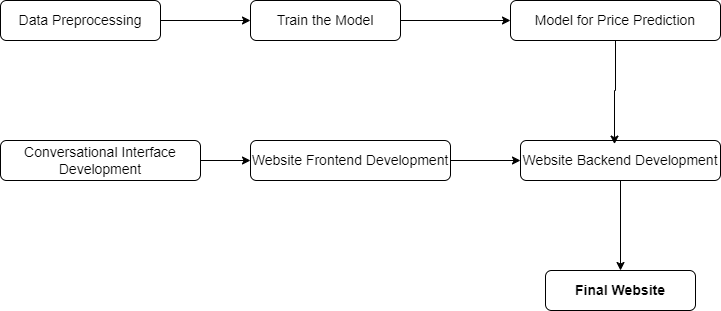
\includegraphics[width=.8\textwidth]{./Flowchart2.png}
    \caption{Solution Flowchart}
    \label{fig:your-label}
\end{figure}
\vspace{\baselineskip} 
The first phase of the project is to find an appropriate dataset and perform data preprocessing. Datasets can be accessed from various websites, such as Kaggle. Python libraries, including Pandas and NumPy, can be used for this preprocessing. 
\newline

The second phase of the project is to train the model. The Scikit-learn library can be used for implementing machine learning regression algorithms, while TensorFlow and Keras can be used for training the dataset using neural networks.
\newline

The third phase of the project is to compare the performance of different algorithms using performance metrics such as Mean Absolute Error (MAE) and select the most accurate algorithm. This chosen algorithm will then be used to train the final model.
\newline

The fourth phase of the project is to develop the Conversational Interfaces. NLP tools like Rasa can be used for this.
\newline
\newline
The fifth phase focuses on developing the frontend of the website, which involves designing and implementing the user interface (UI) for the conversational interface. This will include a Chat Interface: A conversational UI where users can interact with the system through natural dialogue. This interface will guide users in providing necessary details about their cars and receiving price predictions. The UI can be implemented using web development tools such as HTML, CSS, JavaScript, and React.js
\newline

The sixth phase of the project is to develop the backend of the website. This can be implemented using Python frameworks such as Flask or Django.
\newline

The seventh and final phase of the project involves integrating the frontend and backend through API calls. Following integration, testing will be conducted using various test cases. Finally, documentation for the project will be prepared.

\newpage
\section*{Exepected Outcomes}
	\begin{itemize}
		\item The conversational interface will effectively interact with users, guiding them through the process of providing necessary car details in a natural and engaging manner.
		\item A predictive model that provides accurate predictions based on user inputs.
		\item Successful integration of the frontend and backend.

	 \end{itemize}

\section*{Tentative Timeline}
\begin{tabular}{|c|p{7cm}|c|}
\hline
\textbf{PHASE} & \textbf{DESCRIPTION} & \textbf{TIMELINE} \\ \hline
1 & Finalizing project Design \& Module division & September 4 - September 10 \\ \hline
2 & Dataset collection and pre-processing & September 11 - September 18 \\ \hline
3 & Train Model and Compare Algorithm Performance & September 19 - September 30 \\ \hline
5 & Conversational Interface development & October 1 - October 19 \\ \hline
6 & Frontend Development & October 20 - November 4 \\ \hline
7 & Backend Development & November 5 - November 16 \\ \hline
8 & Integration, Testing, and Documentation & November 17 - November 20 \\ \hline
\end{tabular}


\begin{thebibliography}{9}
\bibitem{varshitha2022}
J. Varshitha, K. Jahnavi, and C. Lakshmi, "Prediction Of Used Car Prices Using Artificial Neural Networks And Machine Learning," \textit{2022 International Conference on Computer Communication and Informatics (ICCCI)}, Coimbatore, India, 2022, pp. 1-4, doi: 10.1109/ICCCI54379.2022.9740817.


\bibitem{kathiravan2023}
M. Kathiravan, M. Ramya, S. Jayanthi, V. V. Reddy, L. Ponguru, and N. Bharathiraja, "Predicting the Sale Price of Pre-Owned Vehicles with the Ensemble ML Model," \textit{2023 4th International Conference on Electronics and Sustainable Communication Systems (ICESC)}, Coimbatore, India, 2023, pp. 1793-1797, doi: 10.1109/ICESC57686.2023.10192988.


\end{thebibliography}

\end{justify}

\end{document}
